\documentclass{SBCbookchapter}
\usepackage[utf8]{inputenc}
\usepackage[T1]{fontenc}
\usepackage[brazilian]{babel}
\usepackage{graphicx}
\usepackage[brazilian]{backref}	 % Paginas com as citações na bibl
\usepackage[alf]{abntex2cite}	% Citações padrão ABNT

\usepackage{amsmath}

\usepackage{todonotes}

\author{Márcio Castro, Pedro H. Penna e Alyson D. Pereira\\
\textit{Departamento de Informática e Estatística (INE)}\\
\textit{Universidade Federal de Santa Catarina (UFSC)}
}
\title{Desenvolvimento de Aplicações Paralelas Eficientes com OpenMP}

% Fragmento de Código
\usepackage{listings}
\usepackage[dvipsnames]{xcolor}
\lstset{
  belowcaptionskip=1\baselineskip,
  breaklines=true,
  frame=L,
  xleftmargin=\parindent,
  numbers=left,
  stepnumber=2,
  language=C,
  tabsize=4,
  showstringspaces=false,
  basicstyle=\scriptsize\ttfamily,
  otherkeywords={pragma,
                 omp,
				 parallel,
				 num\_threads},
  keywordstyle=\bfseries\color{blue},
  commentstyle=\itshape\color{gray},
  identifierstyle=\bfseries\color{black},
  stringstyle=\bfseries\color{purple},
}

\begin{document}
\maketitle

\begin{resumo}
Resumo aqui.
\end{resumo}

\section{Introdução}

	Durante as três últimas décadas, os avanços da tecnologia de
	semicondutores e de arquiteturas de computadores permitiram que o
	desempenho de um único processador fosse aumentado com uma taxa anual de
	40\% à 50\% \cite{LARUS08}. Porém, a dissipação de calor do crescente
	número de transistores em um único \emph{chip} começou a limitar o
	aumento da frequência dos processadores. Devido à esse fato, grande
	parte da indústria de semicondutores está agora investindo na produção
	de processadores com diversos núcleos de processamento
	(\emph{multicores}).

	De fato, processadores \emph{multicore} são largamente utilizados nos
	dias de hoje para a Computação de Alto Desempenho \cite{Asanovic09}.
	Porém, observa-se nessas arquiteturas uma grande disparidade entre o
	alto crescimento do número de \emph{cores} por processador e o baixo
	número de conexões entre processadores e o restante dos dispositivos.
	Essa crescente disparidade faz com que o tempo de acesso a um dado
	armazenado na memória seja muito maior que o tempo necessário para
	processá-lo, o que conduz ao conhecido ``\emph{memory wall problem}''
	\cite{McKee-MemWall:2004}. Esse problema é atenuado atualmente através
	do uso de uma hierarquia de memórias \emph{cache} entre os processadores
	e a memória principal, o que permite um acesso mais rápido aos dados e
	melhora o desempenho global.

	A tendência atual da construção de arquiteturas paralelas do tipo
	\emph{multicore} é de um crescimento contínuo do número de \emph{cores},
	resultando em arquiteturas compostas por dezenas ou até mesmo milhares
	de cores. Essa tendência é confirmada pelo \emph{website}
	TOP500\footnote{\url{http://www.top500.org}} (Figura~\ref{fig:top500}),
	o qual provê um ranking atualizado dos 500 supercomputadores mais
	poderosos do mundo. Nessas arquiteturas o problema de escalabilidade é
	ainda maior, pois centenas ou milhares de processos (ou \emph{threads})
	em execução simultânea disputam acesso a diversos recursos
	compartilhados como por exemplo \emph{cores}, memória principal,
	memórias \emph{cache}, entre outros.

	\begin{figure}[h]
		\centering
		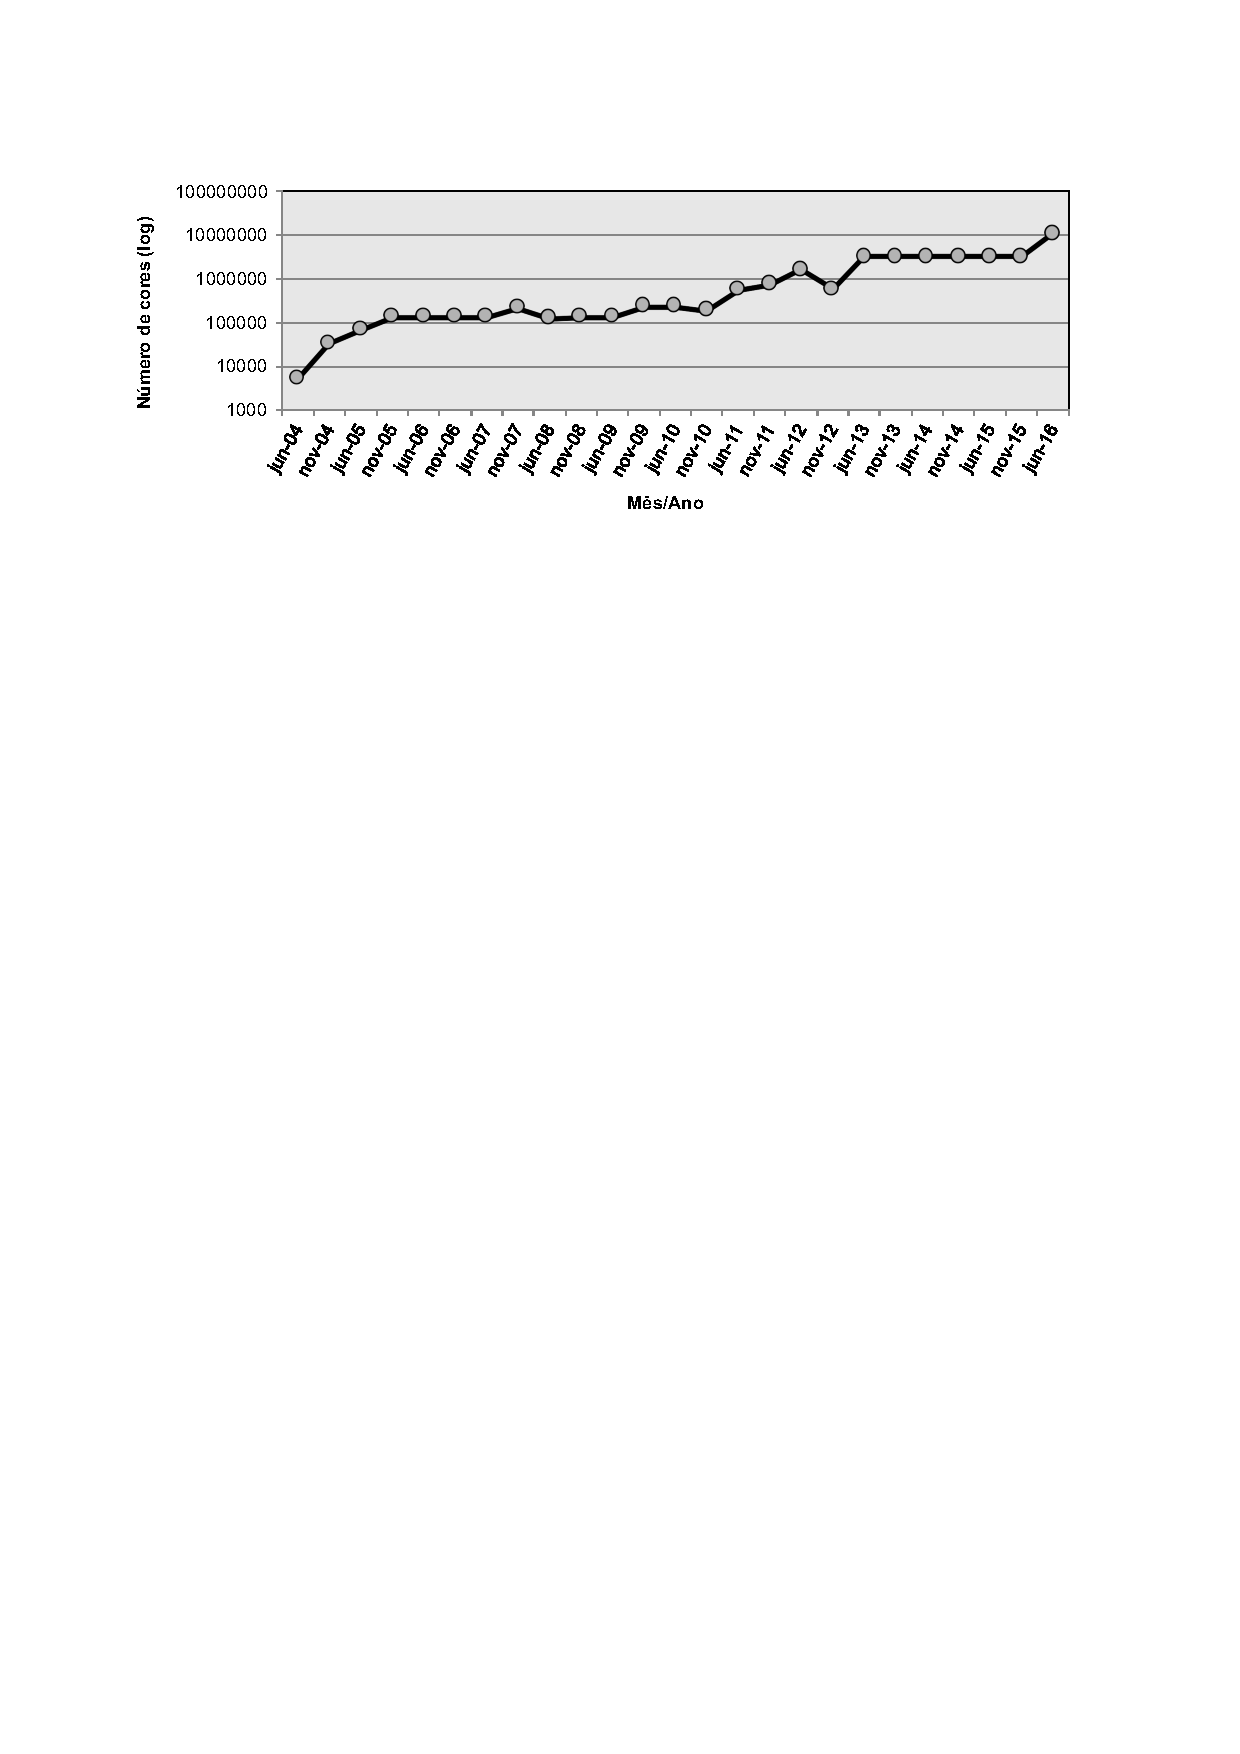
\includegraphics[width=13cm, height=!]{img/cores-top500.pdf}
		\caption{Número total de núcleos de processamento (\emph{cores}) dos supercomputadores mais poderosos relacionados na lista TOP500.}
		\label{fig:top500}
	\end{figure}

	O desenvolvimento de aplicações paralelas eficientes é um requisito
	obrigatório para que seja possível utilizar todo o potencial dessas.
	Para atingir esse objetivo é necessário o uso de modelos de programação
	paralela. Idealmente, esses modelos devem oferecer um nível de abstração
	alto aos desenvolvedores. Ao mesmo tempo, eles devem fornecer mecanismos
	eficientes para a criação, gerenciamento e orquestração de
	\textit{threads} ou processos.

	Nesse capítulo será apresentado um dos modelos de programação paralela
	muito utilizados na academia e na indústria denominado OpenMP. Esse
	modelo oferece diretivas de compilação que permitem realizar a
	paralelização de trechos de código de maneira transparente. O OpenMP
	oferece uma Interface de Programação de Aplicações (\textit{Application
	Programming Interface} -- API) bastante completa para paralelização de
	aplicações para arquiteturas de memória compartilhada. Nesse tipo de
	arquitetura, diversos processadores ou \textit{cores} tem acesso a uma
	memória principal compartilhada em um único espaço de endereçamento. A
	Figura~\ref{fig:arquitetura-multicore} apresenta uma visão geral de uma
	arquitetura de memória compartilhada.

	\begin{figure}[h]
		\centering
		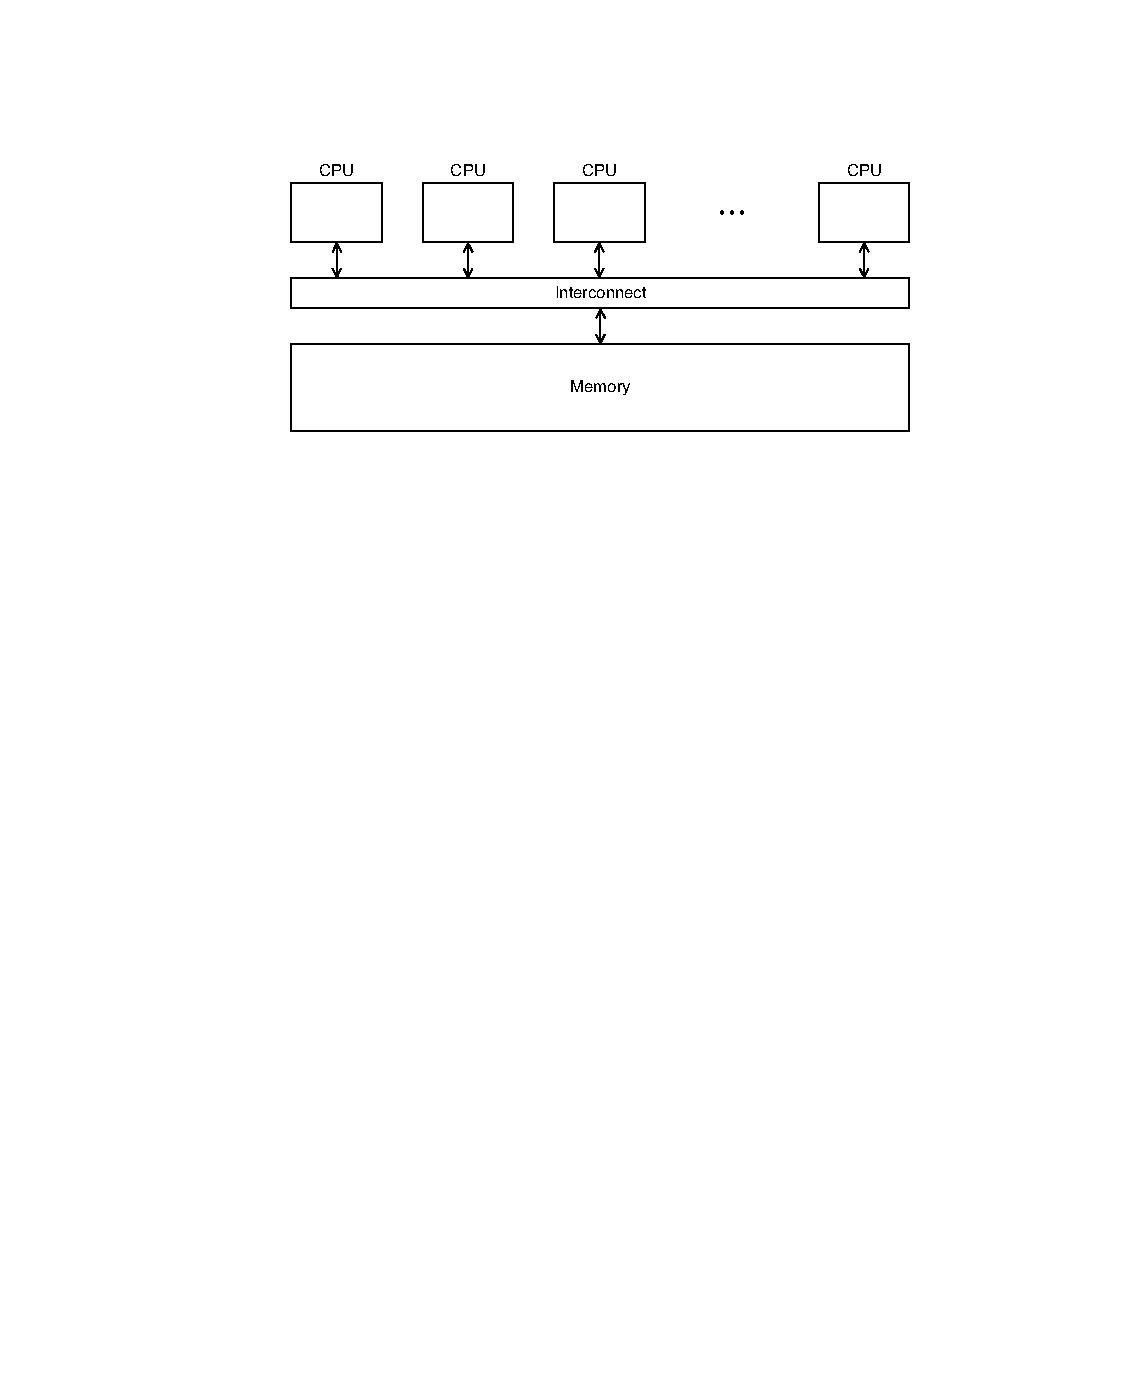
\includegraphics[width=10cm, height=!]{img/arquitetura-multicore.pdf}
		\caption{Exemplo de uma arquitetura de memória compartilhada.}
		\label{fig:arquitetura-multicore}
	\end{figure}

	Existem duas grandes classes de arquiteturas de memória compartilhada. A
	principal diferença entre elas está relacionado ao tempo de acesso dos
	processadores à memória principal. Em arquiteturas do tipo
	\textit{Uniform Memory Access} (UMA), o tempo de acesso entre o
	processador ou \textit{core} e a memória principal é constante. Por
	outro lado, em arquiteturas do tipo \textit{Non-Uniform Memory Access}
	(NUMA) o tempo de acesso entre o processador ou \textit{core} não é
	constante. A diferença no tempo de acesso vem do fato de que cada
	processador ou \textit{core} tem acesso a bancos de memória local
	(próximos a ele) e também a bancos de memória remotos (distantes a ele
	mas próximos de outro processador ou \textit{core}). Nesse sentido, o
	tempo de acesso à memória principal pode ser pequeno (acesso a um banco
	de memória local) ou grande (acesso a um banco de memória remoto),
	dependendo da distância entre o processador ou \textit{core} e o banco
	de memória que esse processador ou \textit{core} está acessando.
	Arquiteturas utilizadas em \textit{notebooks}, \textit{desktops} ou em
	pequenos servidores que contenham poucas dezenas de \textit{cores} são
	do tipo UMA. Porém, arquiteturas paralelas mais complexas que possuem
	várias dezenas de \textit{cores} são normalmente do tipo NUMA.

\section{Conceitos Básicos}

	Essa seção irá abordar os conceitos básicos de programação paralela com
	OpenMP. Primeiramente, será apresentado o modelo base dessa API, em
	seguida será apresentada a primitiva básica para a criação de regiões
	paralelas no código com as formas de compartilhamento de dados
	oferecidas pelo OpenMP.

	\subsection{Modelo Fork-Join}

		% Descrição
		O OpenMP segue o modelo Fork-Join de execução paralela, que é
		ilustrado na Figura (??). Nesse modelo, o programa inicia sua
		execução com uma única thread, denominada \textit{master thread}. A
		\textit{master thread} executa sequencialmente até encontrar uma
		região paralela, definida pela diretiva \texttt{omp parallel}
		(Figura (??)). Nesse ponto, a \textit{master thread} cria um grupo
		de threads trabalhadoras, denominadas \textit{worker threads}
		(Figura (??)), e cada \textit{worker thread} executa então os
		comandos delimitados pela região paralela. Ao concluirem seu
		trabalho, as \textit{worker threads} sincronizam suas atividades e
		terminam (Figura (??)). A \textit{master thread} retoma então a
		execução sequencial do programa até que uma nova região paralela
		seja encontrada, momento em que todo esse processo se repete
		novamente.
		
		% Comentários
		Como observação, é importante deixar claro que a \textit{master
		thread} também executa os comandos na região paralela. Assim, se
		quatro \textit{worker threads} são criadas pela \textit{master
		thread}, um total de cinco threads irão executar a região paralela.
		No entanto, o é possível fazer uso de estruturas condicionais
		alinhadas a funções internas do OpenMP para definir uma execução de
		comandos diferentes para a \textit{master thread}. Esse assunto será
		abordado mais adiante, na Seção \ref{section: sincronizacao}. Por
		fim, vale ressaltar que, em implementações modernas do OpenMP, a
		criação das estruturas internas para gerência das threads em regiões
		paralelas é feita uma única vez, quando a primeira região paralela é
		encontrada. Dessa forma, a sobrecarga imposta na aplicação não
		cresce linearmente com o número de regiões paralelas nela presente.

	\subsection{Regiões Paralelas e Compartilhamento de Dados}

		% Descrição.
		A definição de regiões paralelas no OpenMP é feita através da
		diretiva \texttt{omp\_parallel}, como é ilustrado no Fragmento de
		Código (??). Nesse exemplo, assim que a a \textit{master thread}
		atinge a região paralela (linhas 7 a 12), ela cria um grupo de
		\textit{worker threads} para executar os comandos especificados. Ao
		final da região paralela, uma barreira implícita força a
		sincronização das threads.
		
		% Controle do Número de Threads
		Por padrão, o número de threads no grupo que executará uma região
		paralela será igual ao número de núcleos de processamento no
		processador. No entanto, esse fator pode ser controlador através da
		cláusula  \texttt{num\_threads())}, pela invocação da função
		utilitária \texttt{omp\_set\_num\_threads()}, ou então pela
		definição da variável de ambiente \texttt{OMP\_NUM\_THREADS}. No
		grupo, a \textit{master thread} possui o identificador zero, e o
		identificar das demais threads pode ser recuperador através da
		função utilitária do OpenMP \texttt{omp\_get\_thread\_num()}.

		% Controle de Escopo de Dados 
		Variáveis declaradas fora da região paralela são compartilhadas entre
		todas as threads por padrão. No entanto, a cláusula \texttt{private()}
		pode ser usada para a especificação de variáveis locais privadas, e a
		diretiva \texttt{omp threadprivate} pode ser empregada para a definição
		de variáveis globais privadas. Alternativamente, é possível alterar o
		comportamento padrão para variáveis locais através da cláusula
		\texttt{default()}, definindo todas elas como privadas, e então
		especificar	as variáveis locais compartilhadas pela cláusula
		\texttt{shared()}.

		% Programação de Alto Desempenho
		O uso dos mecanismos apresentados anteriormente é fundamental no
		desenvolvimento de aplicações paralelas eficientes. O ajuste do
		número de threads em uma região paralela evita o desperdício de
		recursos computacionais e possibilita um ajuste da granularidade de
		tarefas. A identificação de threads é necessária para a correta
		coordenação e atribuição de tarefas em uma aplicação. Por fim,
		mecanismos de controle de escopo de dados são inerentemente
		necessários em aplicações paralelas.

\begin{lstlisting}[frame=single]
void sayhello(int nthreads)
{
	void tids[nthreads]

	/* Cria threads. */
	#pragma omp parallel num_threads(nthreads)
	{
		int tid;

		tid = omp_get_thread_num();
		tids[tid] = tid;
	}

	/* Imprime IDs das threads. */
	for (int i = 0; i < nthreads; i++)
		printf("thread %d: my ID is %d\n", i, tids[i]);
}
\end{lstlisting}

\section{Paralelismo de Dados e Diretivas OpenMP}

	% Visão Geral
	No OpenMP, o paralelismo de dados é explorado através de diretivas
	para paralelização de laços. Nessa seção, o uso dessas diretivas para o
	projeto de aplicações no projeto de aplicações paralelas será discutido.
	Primeiro, serão apresentadas as diretivas que possibilitam explorar o
	paralelismo de dados. Em seguida, as estratégias de escalonamento
	disponíveis no OpenMP são apresentadas, assim como suas vantagens e
	desvantagens. Por fim, os mecanismos de redução oferecidos pela API são
	introduzidos.

	\subsection{Paralelização de Laços}
	\label{subsection: paralelização de lacos}

		% Visão Geral
		Duas diretivas de paralelização de laços estão disponíveis no
		OpenMP: \texttt{omp for} e \texttt{omp parallel for}. A primeira,
		diretiva instrui que as iterações do laço seguinte de uma região
		paralela devem ser distribuídas entre as threads do grupo em questão
		e, então, executadas em paralelo. A segunda diretiva tem o mesmo
		efeito, porém não necessita que o laço esteja dentro de uma região
		paralela. O Fragmento de Código (??) ilustra o uso dessa última
		diretiva na paralelização do algoritmo clássico de multiplicação de
		matrizes. Nesse exemplo, um grupo de threads é criado para
		executar os comandos do laço da linha $9$. Cada thread
		recebe um conjunto distinto de iterações e, assim, a
		computação é efetuada em paralelo. 

\begin{lstlisting}[frame=single]
struct matrix *matrix_mult(struct matrix *a, struct matrix *b)
{
	struct matrix *c;

	c = matrix_create(a->nrows, b->ncols);

	/* Multiplica matrizes. */
	#pragma omp parallel for 
	for (int i = 0; i < a->nrows; i++)
	{
		for (int j = 0; j < a->cols; j++)
		{
			for (int k = 0; k < a->ncols; k++)
				MATRIX(c, i, j) += MATRIX(a, i, k)*MATRIX(b, k, j);
		}
	}

	return (c);
}
\end{lstlisting}

		% Discussão de Granularidade
		Observe que nesse exemplo, assim como em diversas outras aplicações que
		também exploram o paralelismo de dados presente em laços, a diretiva de
		compilação também poderia ter sido colocada no segundo laço mais externo
		sem perda de semântica. No entanto, as duas abordagens se difeririam
		quanto à granularidade de paralelização. Na primeira abordagem, o grão
		de trabalho entregue a cada thread é mais grosso, enquanto na segunda
		abordagem o grão de trabalho é mais fino. O controle de granularidade
		consiste em uma técnica importante no projeto de aplicações paralelas
		eficientes, pois tanto possibilita que a localidade temporal e de dados
		sejam exploradas; quanto sobrecargas de sincronização e irregularidades na
		computação sejam contornados. Na Seção (??) as peculiaridades desse
		assunto serão discutidas em maiores detalhes.

		\begin{figure}
			\centering
			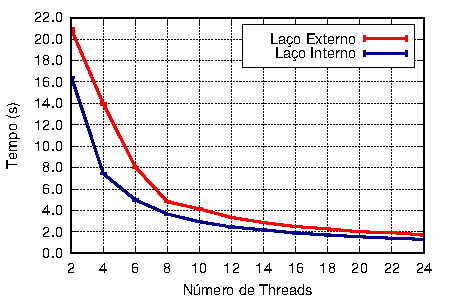
\includegraphics[width=0.50\textwidth]{img/matrix-mult}
		\end{figure}

		% Análise de Desempenho
		Para ilustrar o impacto no desempenho que cada uma dessas abordagens
		teriam no algoritmo clássico de multiplicação de matrizes, foram
		conduzidos experimentos em uma máquina SMP com 24 núcleos ($2 \times$
		Xeon X7). Nesses experimentos, foi fixado o tamanho da matriz de entrada
		em $1680 \times 1680$ e foi variado o número de threads de $2$ a $24$.
		Com esse simples experimento, pode-se constatar que, para a plataforma e
		carga considerados, a abordagem de paralelização mais fina conduz a um
		melhor desempenho. Ademais, para o tamanho da matriz de entrada
		estudado, percebe-se que o ganho obtido com $14$ threads ou mais não é
		significante maior do que com $12$ threads. Esse resultado, indica então
		que utilizar mais que $12$ threads para esse tamanho de problema
		significa um desperdício de recursos computacionais.

		\todo[inline]{Inserir resultados de estatística do uso de caches.}

	\subsection{Escalonamento de Iterações}
	\label{subsection: escalonamento de iteracoes}

		% Aplicações Regulares
		O escalonamento de iterações diz respeito ao modo como iterações de
		um laço paralelo são atribuídas às threads de um grupo. Por padrão,
		no OpenMP, o escalonamento de iterações é feito estaticamente e em
		blocos (ou \textit{chunks}) de mesmo tamanho. Para aplicações que
		possuem um padrão de computação regular, isto é, o tempo de
		computação para cada iteração do laço paralelo é o mesmo, essa
		estratégia conduz a ganhos de desempenhos satisfatórios, pois esse
		particionamento estático é capaz de distribuir a carga de trabalho
		de forma uniforme entre as threads. O algoritmo de multiplicação de
		matrizes apresentado na seção anterior exemplifica a classe de
		algoritmos regulares. No caso, a carga de trabalho entregue a cada
		thread é constate e proporcional a:
		%
		\begin{align*}
			\text{Carga de Trabalho} = \dfrac{\text{Numéro de Linhas na Matriz}}%
			                                 {\text{Número de Threads}}
		\end{align*}

		% Aplicações Irregulares
		No entanto, para aplicações que possuem um caráter irregular de
		computação, isto é, o tempo de computação para cada iteração no laço
		paralelo difere; ou então para aplicações regulares que possuem
		afinidade de memória entre diferentes iterações; essa estratégia não
		se mostra eficiente e escalável~[??]. Então, para atacar esses
		cenários problemáticos, o OpenMP disponibiliza a cláusula
		\texttt{schedule}, que possibilita: (i) controlar qual será a
		estratégia de escalonamento que será empregada para escalonar as
		iterações de um laço paralelo; e (ii) definir quantas iterações são
		escalonadas por vez a uma única thread. A estratégia de
		escalonamento permite contornar o problema do desbalanceamento de
		carga presente em aplicações irregulares, equanto o controle do
		tamanho de bloco de iterações a ser escalonado por vez permite
		ajustar a granularidade de paralelização, possibilitando assim que a
		afinidade de memória existente entre iterações seja explorada. O
		tamanho de bloco de iterações pode ser escolhido arbitrariamente,
		já a estratégia de escalonamento pode ser selecionada dentre as
		seguintes, em uma implementação padrão do OpenMP:
		%
		\begin{itemize}
			\item static: particiona igualitariamente as iterações de um
			laço paralelo em chunks de iterações. A atribuição de chunks
			é feita em tempo de compilação e nenhuma sobrecarga é
			adicionada a aplicação. Essa estratégia é indicada para
			aplicações regulares.
			
			\item dynamic: atribui chunks de iterações às threads sob
			demanda em tempo de execução. Para que a atribuição seja feita
			dinamicamente, durante a execução da aplicação, uma sobrecarga
			gerência é introduzida na aplicação. Essa estratégia é indicada
			para uso em aplicações com alto grau de irregularidade.

			\item guided: similar à estratégia dynamic, porém o tamanho do
			chunk de iterações decresce com o tempo. Essa estratégia
			também impões uma sobrecarga na execução da aplicação, porém
			relativamente menor que a estrátégia dynamic. Essa
			estratégia é indicada para uso em aplicações com baixo e
			médio graus de irregularidade, onde as iterações iniciais
			do laço paralelo podem ser atribuídas em chunks maiores, e
			assim alguma sobrecarga de sincronização evitada.
		\end{itemize}
		
		% Exemplo
		O Fragmento de Código (??) ilustra o uso desses dois mecanismos na
		paralelização do algoritmo clássico para multiplicação de matrizes
		esparsas, um típico representante de uma aplicação irregular. Nesse
		exemplo, o escalonamento de iterações é feito em blocos de tamanho
		um e usando a política Dynamic. Uma avaliação quantitativa do
		desempenho dessa estratégia nessa aplicação particular, frente às
		estratégias Static e Guided, é apresentada na Figura (??).
		Experimentos foram conduzidos em uma máquina SMP com 24 cores ($2
		\times$ Intel Xeon X7) para uma matriz de tamanho $1680 \times
		1680$. Para essa aplicação, tamanho de problema e plataforma, a
		análise dos resultados revela que a estratégia de escalonamento
		Dynamic conduz a maiores ganhos de demsepenho e se mostra mais
		escalar quando comparada à política Static e Guided.

		\todo[inline]{Inserir resultados matriz esparsa}.

\begin{lstlisting}[frame=single]
struct matrix *sparsematrix_mult(struct matrix *a, struct matrix *b)
{
	struct matrix *c;

	c = matrix_create(a->nrows, b->ncols);

	/* Multiplica matrizes esparsas. */
	#pragma omp parallel for 
	for (int i = 0; i < a->nrows; i++)
	{
		for (int j = 0; j < a->cols; j++)
		{
			for (int k = 0; k < a->ncols; k++)
			{
				if (MATRIX(a, i, k) != 0)
					MATRIX(c, i, j) += MATRIX(a, i, k)*MATRIX(b, k, j);
			}
		}
	}

	return (c);
}
\end{lstlisting}

	\todo[inline]{Discussão sobre tamanho do chunk e overhead.}

	\subsection{Redução de Operações}
	\label{subsection: reducao de operacoes}

\section{Paralelismo de Tarefas e Diretivas OpenMP}

	O paralelismo de tarefas será explorado através do estudo das diretivas
	de compilação disponíveis no OpenMP para paralelização de trechos de
	códigos. Serão discutidas duas construções: seções (\texttt{omp
	sections}) e tarefas (\texttt{omp task} e \texttt{omp taskwait}). A
	utilização de tarefas será abordada com o auxilio de problemas
	recursivos clássicos.

\section{Sincronização}
\label{section: sincronizacao}

	Nesse capítulo serão discutidas as diretivas de sincronização de threads
	disponíveis no OpenMP: serialização de código (\texttt{omp single} e
	\texttt{omp master}), exclusão mútua (\texttt{omp critical}) e barreiras
	(\texttt{omp barrier}).

\section{Conclusão}

	Esse capítulo apresentará um apanhado geral do minicurso, ressaltando os
	principais pontos abordados no texto.

\bibliography{referencias}

\end{document}
